\graphicspath{{main/introduction/graphics/}}

\section{Technical Background}

\subsection{Real-Time}
A real-time system is defined as a system which requires correct logical operation with completion in a configured deadline. This is in contrast to a non-real-time system which correct operation is desired but lacks configured deadlines. \autocite{kaviRealTimeSystems2009}

These real-time systems can be categorised into hard and soft. Hard real-time systems contain strict timing constraints, where a response must be calculated in a specified time-frame and a missed deadline could result in a catastrophic outcome. Soft real-time systems also have timing constraints, but a missed deadline should not result in a catastrophic outcome.

% some equations for the hard vs soft
% some examples of what is required for hard and soft systems

Typical hard real-time systems include aircraft or robotic control computers and soft real-time systems include media players or gaming computers. Soft real-time systems can be used in control applications, but the soft timing must be considered in the system design.

\subsection{Control Systems}
A control system
Differential equation

% open loop and closed loop

\subsection{Operating Systems}
An Operating System (OS) is a piece of software that controls the execution of application programs on a system. Usually this involves managing resource allocations, such as a processor execution time, memory usage and generic inputs/outputs. \autocite{stallings2018operating}

In order to develop a real-time applications with an OS, a RTOS (Real-Time Operating System) is usually required. This is to ensure the time deadlines of an application are inforced.

Hard real time operating system are designed to run applications with absolute timing
Worst-Case Execution Time
Assigned a relative deadline, all tasks must complete in their deadline.
Modelled mathematically to ensure that all tasks run to completion

Define the maxiumum delay after a deadline

Scheduling
Memory
UNIX, POSIX

\subsection{Virtualization}
Virtual machines create isolated or emulated computing environments by abstracting resources within a physical machine \autocite{liSurveyVirtualMachine2010}. Software known as hypervisors can provide this abstraction layer \autocite{rountreeSystemSecurity2011}. Hypervisors that directly access the underlying machine resources are known as Type 1 \textit{bare metal} hypervisors, examples include Hyper-V \autocite{phsteeHyperVArchitecture2023}, Xen \autocite{xenprojectVirtualization}, ESXi \autocite{vmwareWhatESXI} or KVM \autocite{redhatWhatKVM}. 

\begin{figure}[ht]
    \centering
    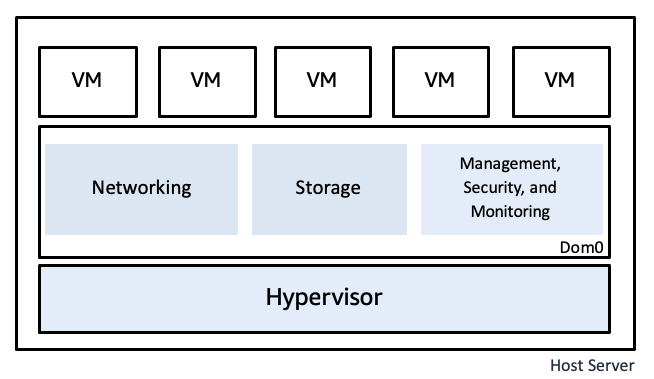
\includegraphics[width=8cm]{awsWhatDifferenceType}
    \caption[Type 1 hypervisor architecture \autocite{awsWhatDifferenceType}]
    {Type 1 hypervisor architecture \autocite{awsWhatDifferenceType}}
    \label{fig:awsWhatDifferenceType}
\end{figure}

A fully virtualized Type 1 hypervisor (KVM) emulates privileged instructions and I/O operations, abstracting the hardware resources from the virtual machine. The guest operating system therefore requires no modifications as it is unaware of the virtualisation. In contrast, with paravirtualizaion the guest operating system requires significant modifications and is aware of the underlying hardware. Xen uses paravirtualizaion and a modified version of the Linux kernel can run as a guest OS. Hardware assisted virtualisation uses additional CPU instructions to isolate virtual machines in a hypervisor, for example AMD-V \autocite{liSurveyVirtualMachine2010}.

Type 2 hypervisors negotiate resource allocation with the operating system, which makes the process slower and less efficient \autocite{awsWhatDifferenceType} such as VMware Workstation \autocite{vmwareWhatHypervisorVMware}.

\subsection{Mixed Criticality}


\subsection{Middleware}

%  generic embedded middleware

% aircraft focused middleware (IMA DIMA)

\subsection{Software Updates}
